\chapter{REVISÃO DE LITERATURA}\label{chap:fundamentacaoTeorica}

Para o presente trabalho, em decorrência dos instrumentos e sensores escolhidos, devemos colher na literatura as equações e formalismos que descrevem o movimento e a orientação dos corpos no espaço, bem como as relações com as forças envolvidas. Além da literatura básica sobre mecânica v.~\cite{Goldstein1980}, robótica v.~\cite{Craig2014} e controle v.~\cite{Ogata2010}, os temas são mais bem explorados na literatura sobre controle de aeronaves e mísseis v.~\cite{Henderson1997}, \cite{Stevens2016}, \cite{Blakelock1991} ou sobre navegação inercial v.~\cite{Stovall1997}, \cite{Weston2004}, \cite{Wang2021} e~\cite{Haoran2019}

No particular, empregaremos em grande parte as convenções e equações utilizadas em~\cite{Stevens2016}, que acreditamos dar um tratamento mais direto e acessível a esses temas.

\section{Notação e convenções}

Neste trabalho utilizamos um modelo de mundo tridimensional e mecânica clássica.  Nosso espaço é estruturado por três eixos ortogonais \(x\), \(y\), \(z\) (\(1, 2, 3\)) onde uma posição é dada por um vetor tridimensional. Descreveremos a atitude e o movimento de um corpo rígido sobre a superfície oblata e girante da Terra. Não obstante, serão empregadas aproximações sobre uma pequena área para uma Terra plana, estacionária e constante, que basta\footnotemark{} para os nossos propósitos. Para simbologia, acompanhamos \cite{Stevens2016}:

\begin{align*}
    \mathbf{p}_{A/B} &\equiv
    \text{ vetor posição do ponto A em relação ao ponto B} \\
    \mathbf{v}_{A/i} &\equiv
    \text{ vetor velocidade do ponto \(A\) tomada no sistema \(F_{i}\)} \\
    ^{b}\mathbf{\dot{v}}_{A/i} &\equiv
    \text{ vetor derivada de \(\mathbf{v}_{A/i}\) tomada no sistema \( F_{b}\)} \\
    \mathbf{v}^{c}_{A/i} &\equiv \left( \mathbf{v}_{A/i} \right)^{c} \equiv
    \text{ conjunto dos componentes de \(\mathbf{v}_{A/i}\) expressos no sistema \(c\)} \\
\end{align*}

Componentes de vetores terão índices para indicar o sistema de coordenadas ou serão denotados pelo símbolo de vetor com índices \(x\), \(y\), e \(z\) para indicar as coordenadas, exceto quando indicado pelo símbolo transposto, e todos vetores são do tipo vetor coluna. Acompanhando~\cite{Stevens2016}, por exemplo:
\begin{align*}
    &\mathbf{p}^{b}_{A/B} = \begin{bmatrix}x_{b} \\ y_{b} \\ z_{b}\end{bmatrix}&
    \text{ ou }&
    &\mathbf{v}^{b}_{A/i} = \begin{bmatrix} v_{x} \\ v_{y} \\ v_{z} \end{bmatrix} = \begin{bmatrix} v_{x} & v_{y} & v_{z} \end{bmatrix}^{T}
\end{align*}

\footnotetext{A título de advertência, o assunto não é simples, com diversos formalismos possíveis, um campo fértil para confusão. Por exemplo, a atitude de um corpo pode ser descrita em três dimensões com ângulos de Euler ao menos em doze sequências de rotações anti-horárias distintas, não intercambiáveis, ou ainda pode ser descrita em quatro dimensões com o uso do quaternion, conforme observamos em~\cite{Henderson1997}. Além disso, é importante separar a orientação relativa do nosso espaço tridimensional em abstrato, do eixo de referência em relação ao nosso espaço abstrato, e do sistema móvel que pretendemos descrever em relação ao sistema de referência. No presente trabalho adotaremos um único formalismo que atende aos nossos propósitos limitados, e remetemos o leitor às fontes para aprofundamento do assunto.}

\section{Descrevendo a atitude de um corpo}

Descrevemos a atitude de um robô em ângulos de Euler na sequência \(z\), \(y\), \(x\) (3, 2, 1) que leva de um sistema de referência fixo na Terra até um sistema fixo no corpo do robô. Escolhemos o sistema (\(ned\)) - ``North-East-Down'' (Norte, Leste, Abaixo) com o eixo \(x\) apontando par o Norte, o eixo \(z\) Abaixo, o eixo \(y\) completando o sistema de coordenadas, e o sistema (\(frd\)) - ``Front-Right-Down'' (Avante, Direita, Abaixo), fixo no robô, com eixos, respectivamente, (\(x\),\(y\),\(z\)), sendo o Avante alinhado à \emph{linha de referência longitudinal} do robô, com ``Avante'' e ``Abaixo'' situados no plano de simetria, e o eixo Direito completando o sistema. Adotamos, ainda a convenção de rotações anti-horárias (regra da mão direita).

Desse a modo, a sequência de rotações que leva do sistema de referência \(ned\) para o sistema \(frd\) no corpo é dada por:
\begin{enumerate}
    \item Rotação anti-horária sobre eixo \(z\), ou \(\psi\) positivo (\textit{``compass heading''})
    \item Rotação anti-horária sobre novo eixo \(y'\), ou \(\theta\) positivo (\textit{pitch})
    \item Rotação anti-horária sobre novo eixo \(x''\), ou \(\phi\) positivo (\textit{roll})
\end{enumerate}

Esta sequência de rotações é normalmente denominada \emph{``yaw, pitch, roll''} (guinada, arfada e rolagem), partindo do sistema de referência.

Podemos escrever as matriz de rotação abreviando co-seno por \(c\) e seno por \(s\). Esta matriz representa uma transformação padrão que será utilizada ao longo do texto, acompanhando~\cite{Stevens2016}:

\begin{align*}
    C_{f\!r\!d\!/\!n\!e\!d} =
    \begin{bmatrix}
        1               &  0            &  0             \\
        0               &  \cos{\phi}   &  \sin{\phi}    \\
        0               & -\sin{\phi}   &  \cos{\phi}
    \end{bmatrix}
    \begin{bmatrix}
        \cos{ \theta}   &  0            & -\sin{\theta} \\
        0               &  1            &  0            \\
        \sin{ \theta}   &  0            &  \cos{\theta}
    \end{bmatrix}
    \begin{bmatrix}
        \cos{\psi}      &  \sin{\psi}   &  0             \\
       -\sin{\psi}      &  \cos{\psi}   &  0             \\
        0               &  0            &  1
    \end{bmatrix}
\end{align*}
\begin{align} \tag{1.3-10}
    C_{f\!r\!d\!/\!n\!e\!d} &=
    \begin{bmatrix}
        c\theta c\psi   & c\theta s\psi & -s\theta    \\
        \left(-c\phi s\psi + s\phi s\theta c\psi \right) 
        &  \left( c\phi c\psi + s\phi s\theta s\psi \right) 
        &  s\phi c\theta                                 \\
        \left( s\phi s\psi + c\phi s\theta c\psi \right) 
        &  \left( -s\phi c\psi + c\phi s\theta s\psi \right) 
        & c\phi c\theta
    \end{bmatrix}
\end{align}

O intervalo de validade para o qual os ângulos de rotação são bem definido\footnotemark{} é:
\begin{align*}
    -\pi  < \phi \leq \pi \\
    -\frac{\pi}{2} \leq \theta \leq \frac{\pi}{2} \\
    -\pi < \psi \leq \pi
\end{align*}

\footnotetext{A título de exemplo, ponderamos que caso o ângulo \( \theta \) fosse definido no intervalo de \( \pm 180^{\circ} \) o veículo estaria apontando para o Sul com os ângulos \(\phi\) e \(\psi\) em \( 0^{\circ}\) o que é indesejável pois pode confundir a interpretação.}

\section{Cinemática Rotacional}

Aqui definiremos a derivada de um vetor, mostraremos como ela depende do sistema de referência do observador, e relacionamos as derivadas de um vetor, tomadas em dois sistemas de referência distintos, através do vetor velocidade angular relativa entre esses dois sistemas.

Genericamente a derivada de um vetor é similar à de um escalar~\cite{Stevens2016}:
\begin{equation*}
    \frac{\mathrm{d}}{\mathrm{d}t} \mathbf{p}_{A/B} =  \lim_{\delta t \rightarrow 0 } \begin{bmatrix}
        \displaystyle\frac{\mathbf{p}_{A/B} (t + \delta t) - \mathbf{p}_{A/B} (t) }{\delta t}
    \end{bmatrix}
\end{equation*}

Este novo vetor decorre das mudanças de módulo e orientação de \(\mathbf{p}_{A/B}\). Sendo \(\mathbf{p}\) um vetor livre (por exemplo, a velocidade) sua derivada independe de sua posição, e as mudanças de comprimento e direção decorram do movimento da ponta de \(\mathbf{p}\) em relação à própria cauda. Seja \(\mathbf{p}\) seja um vetor vinculado a algum sistema (por exemplo, o vetor posição) sua derivada naquele sistema é um vetor livre que corresponde à ponta de \(\mathbf{p}\).

\subsection{Velocidade Angular como Vetor}

Um vetor pode apontar em qualquer direção por meio de uma simples rotação ao longo de um eixo apropriado. A fórmula para essa rotação é descrita em~\cite{Goldstein1980}:

\begin{figure}[h]
    \centering
    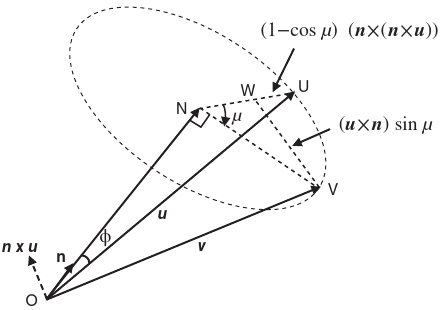
\includegraphics[width=0.5\textwidth, keepaspectratio]{figuras/figure1.2-1.png}\label{fig1.2-1}
    \caption{Rotação de um vetor}\label{fig:rotacao-de-um-vetor}
\end{figure}

Na figura acima, o vetor \(\mathbf{u}\) foi rotacionado para formar o vetor \(\mathbf{v}\) ao definirmos um eixo de rotação ao longo do vetor \(\mathbf{n}\) e realizarmos uma rotação pelo ângulo \(\mu\) ao redor de \(\mathbf{n}\). Estes dois vetores se somam a \(\mathbf{u}\) para obtermos \(\mathbf{v}\), e onde temos que:
    \begin{align*}
     \mathbf{v} &= \mathbf{u} + \left(1 - {\cos{\mu}}\right) \left(\mathbf{n}\!\times\!\left(\mathbf{n}\!\times\!\mathbf{u}\right)\right) - \left(\mathbf{n}\!\times\!\mathbf{u}\right){\sin{\mu}} \tag{1.2-5a}
    \end{align*}
    \begin{align*}
     \mathbf{v} = \left(1 - {\cos{\mu}}\right) \mathbf{n}\!\left(\mathbf{n}\cdot\mathbf{u}\right) + \mathbf{u}{\cos{\mu}} - \left(\mathbf{n}\!\times\!\mathbf{u}\right){\sin{\mu}} \tag{1.2-5b}
    \end{align*}

    As equações acima (1.2-5), às vezes chamadas de \textit{fórmula de rotação}, nos mostram que definindo \(\mathbf{n}\) e \(\mu\) podemos operar sobre \(\mathbf{u}\) com produtos escalares e vetoriais para obter a rotação desejada, independente de sistemas de coordenadas ou magnitude do ângulo.

    Partindo da figura acima, fazemos uma rotação muito pequena \(\delta\mu \ll 1 \text{rad}\), definindo \(\mathbf{v} = \mathbf{u} + \delta \mathbf{u}\), e, aplicando a equação (1.2-5\(a\)) obtemos:
\begin{equation*}
    \delta \mathbf{u} \approx -\!\sin(-\delta\mu)\mathbf{n}\!\times\!\mathbf{u} \approx (\mathbf{n}\!\times\!\mathbf{u})\delta\mu
\end{equation*}

Dividindo por \(\delta t\), no limite onde \(\delta t \rightarrow 0\), definindo \(\mathbf{\omega} \equiv \dot{\mu}\mathbf{n}\), obtemos:

\begin{equation*}
    \dot{\mathbf{u}} = \mathbf{\omega}\!\times\!\mathbf{u}\tag{1.4-1}
\end{equation*}

Esta equação relaciona a velocidade translacional da ponta do vetor \(\mathbf{u}\) ao vetor \(\mathbf{\omega}\). Este vetor \(\mathbf{\omega}\), que denominados \textit{vetor velocidade angular}, constitui-se de um vetor unitário  que define o eixo de rotação, multiplicado pela taxa de rotação. Este é um vetor livre, pode ser trasladado paralelo a si mesmo, e axial, que mudaria de direção caso houvéssemos escolhido uma convenção de sentido horário para a rotação.

Dessa forma podemos associar \(\mathbf{\omega}\) ao sistema de coordenadas fixado no corpo, atribuindo índices que indicam que ele representa a velocidade angular do corpo em relação a outro determinado sistema.

Como vimos, a atitude de um corpo rígido pode ser descrita por uma matriz rotacional variante no tempo, e, pelo teorema de Euler\footnotemark{}, esse o corpo possui um único \emph{eixo instantâneo de rotação} ao qual o vetor velocidade angular é paralelo, e também único.

\footnotetext{\emph{``Euler's Theorem: The general displacement of a rigid body with one point fixed is a rotation about some axis.''} Para uma explicação a respeito, vide~\cite{Goldstein1980}, Capítulo 4.}

\section{Cinemática e Ângulos de Euler}

Um corpo em movimento pode mudar sua atitude, descrita em ângulos de Euler, ao longo do tempo, e neste sentido podemos falar de uma taxa de mudança de cada um desses ângulos de Euler ao longo do tempo. Essas taxas são coisa distintas, é preciso dizer, do vetor velocidade angular do corpo.

Para vincular as taxas de ângulos de Euler, que descrevem a mudança de atitude de um corpo, à sua velocidade angular, procedemos do seguinte modo. Definimos um quadro de referência \(F_{r}\) e um quadro do corpo \(F_{b}\) com vetor velocidade angular relativa \(\omega_{b/r}\) e uma sequencia de ângulos de Euler que define a atitude do corpo, ou seja, a orientação do sistema de coordenadas preso ao corpo em relação ao sistema de referência. Cada taxa de ângulos de Euler informa a direção e magnitude para um determinado vetor velocidade angular sobre um eixo de coordenadas em particular. Esses três vetores somados formam o vetor velocidade angular resultante do veículo cujas taxas de ângulos de Euler estamos tratando. Desse modo podemos encontrar os componentes do vetor velocidade angular resultante \cite{Stevens2016}.

Em outras palavras, movemos sobre a Terra um sistema de coordenada \(frd\) (\emph{``front'', ``right'', ``down''} - frente, direita, abaixo) preso no corpo, com o sistema \(ned\) (\emph{``north'', ``east'', ``down''} - norte, leste abaixo) fixo no quadro de referência, usando uma sequencia ``yaw-pitch-roll'' de ângulos de Euler do sistema \(ned\) para o sistema \(frd\). No caso das equações de Terra plana o sistema \(ned\) é fixado na Terra, e a velocidade angular relativa é aquela do corpo em relação à Terra. Não trataremos aqui do caso mais geral das equações com seis graus de liberdade onde sistema \(ned\) se move sobre a Terra.

As transformações de coordenadas são~\cite{Stevens2016}:

\begin{align*}
    \mathbf{\omega}^{frd}_{b/r} = \begin{bmatrix} \dot\phi \\ 0 \\0 \end{bmatrix}
    + C_{\phi} \begin{pmatrix}
        \begin{bmatrix} 0 \\ \dot\theta \\ 0 \end{bmatrix}
        + C_{\theta}\begin{bmatrix} 0 \\ 0 \\ \dot\psi \end{bmatrix}
    \end{pmatrix}
\end{align*}

\ldots sendo \(C_{\phi}\) e \(C_{\theta}\)  as rotações (anti-horárias) dos planos por cada ângulo de Euler em particular, conforme equação (1.3-10). Multiplicando as matrizes, teremos:

\begin{align} \tag{1.4-3}
    \mathbf{\omega}^{frd}_{b/r} \equiv \begin{bmatrix} P \\ Q \\ R \end{bmatrix}
    = \begin{bmatrix}
        1 & 0 & -\sin{\theta} \\
        0 & \cos{\phi} & \sin{\phi}\cos{\theta} \\
        0 & -\sin{\phi} & \cos{\phi}\cos{\theta}
    \end{bmatrix}
    \begin{bmatrix}
        \dot\phi \\
        \dot\theta \\
        \dot\psi
    \end{bmatrix}
\end{align}

\ldots sendo \(P\), \(Q\), \(R\), os componentes do vetor velocidade angular do corpo espresso no sistema \(frd\), respectivamente, rolagem (\emph{``roll''}), arfada (\emph{``pitch''}) e guinada (\emph{``yaw''}). A transformação inversa é dada por:

\begin{align} \tag{1.4-4}
    \begin{bmatrix}
        \dot\phi \\
        \dot\theta \\
        \dot\psi
    \end{bmatrix}
    =
    \begin{bmatrix}
        1 & \sin{\phi}\tan{\theta} & \cos{\phi}\tan{\theta} \\
        0 & \cos{\phi} & -\sin{\phi} \\
        0 & \frac{\sin{\phi}}{\cos{\theta}} & \frac{\cos{\phi}}{\cos{\theta}}
    \end{bmatrix}
    \begin{bmatrix}
        P \\ Q \\ R
    \end{bmatrix}
\end{align}

Para simplificar, definimos \(\Phi \equiv \left[\phi \theta \psi \right]^T \) e reescrevemos  (1.4-4) assim:

\begin{equation} \tag{1.4-5}
    \Phi = H \left( \Phi \right) \mathbf{\omega}^{frd}_{b/r}
\end{equation}

As equações (1.4-3) e (1.4-4) serão referidas como as equações cinemáticas de Euler, como faz~\cite{Stevens2016}. Note que as matrizes de coeficientes \emph{não são} matrizes ortogonais representando rotações ordinárias de coordenadas. Note ainda que as Equações (1.4-4) e (1.4-4) possuem uma singularidade quando  \(\theta = \pm \frac{\pi}{2}\). Ainda, se essas equações forem utilizadas em uma simulação, as taxas de ângulos de Euler podem integrar para ângulos fora do intervalos de ângulos de Euler, e portanto, seria necessário incluir uma lógica para lidar com essa situação no programa simulador. Não obstante, as equações cinemáticas de Euler são bastante empregadas em simulações.

\section{Equações do movimento}

ADAPTAR DE \cite{Stevens2016}

\subsection{Vector Derivatives and Rotation}

To understand the derivative of a vector, observed from another frame, in relative motion, we can proceed as follows.

Figure 1.4-1 shows a frame \(F_{b}\) in arbitrary motion with respect to another frame \(F_{a}\) and with angular velocity \(\mathbf{\omega}_{b/a}\). Fixed point \(Q\) has translational velocity \(\mathbf{v}_{Q/a}\) with respect to \(F_{a}\), and vector \(\mathbf{p}\) from \(Q\) is the vector of interest. An observer in \(F_{b}\) watching the tip of this vector would see the new vector \(\mathbf{p}_{1}\) corresponding to a nonzero derivative \({^b\dot{\mathbf{p}}}\). An observer in \(F_{a}\) would see, in addition, the effect of the angular velocity of \(F_{b}\) with respect to \(F_{a}\), giving the vector \(\mathbf{p}_{2}\). The \(F_{a}\) observer would also see \(\mathbf{p}_{2}\) translated parallel to itself because of the translational velocity \(\mathbf{v}_{Q/a}\). However, the derivative in \(F_{a}\) is a free vector and this translation does not entail a change in length or direction of \(\mathbf{p}_{2}\). The derivative \(^{a}\dot{\mathbf{p}}\) is obtained by comparing \(\mathbf{p}_{2}\) with \(\mathbf{p}\) as \(\delta t \rightarrow 0\).
\begin{figure}[h!]
    \centering
    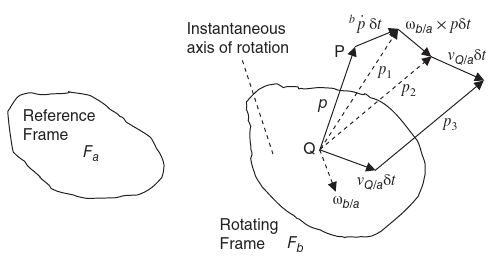
\includegraphics[width=0.5\textwidth, keepaspectratio]{figuras/figure1.4-1.png}\label{fig1.4-1}
    \caption{A vector derivative in a rotating frame.}
\end{figure}
In time \(\delta t\), \(\mathbf{p}_{2} \!-\! \mathbf{p}\) is given by
\begin{equation*}
    \mathbf{p}_{2} - \mathbf{p} = {^{b}\dot{\mathbf{p}}} \delta t + \left( \mathbf{\omega}_{b/a} \! \times \!\mathbf{p} \right) \delta t
\end{equation*}
Dividing by \(\delta t\) and taking the limit as \(\delta t \rightarrow 0\) give
\begin{equation*} \tag{1.4-2}
    {^{a}\dot{\mathbf{p}}} = {^{b}\dot{\mathbf{p}}} + {\mathbf{\omega}_{b/a} \! \times \!\mathbf{p}}
\end{equation*}

Equation (1.4-2) is sometimes called the \textit{equation of Coriollis} (Blakelock, 1965) and will be an essential tool in developing equations of motion from Newton's laws. It is much more general than is indicated above and applies to any physical quantity that has a vector representation. The derivatives need not even be taken with respect to time. Angular velocity can be defined as the vector that relates the derivatives of any arbitraty frames, according to (1.4-2). In the interests of having a vector diagram and intuitive feel, we have derived the equation in a rather restricted fashio. A mro rigorous derivation (with no diagram) has been given by McGill and King( 1992) and a longish derivation with a different kind of diagram by Pestel and Thompson (1968).

Some formal properties of the angular velocity vector are:
\begin{enumerate}[label=\alph*)]
\item It is a unique vector that relates the derivatives of a vector taken in two different frames.
\item It satisfies the relative motion condition \(\mathbf{\omega}_{b/a} = - \mathbf{\omega}_{a/b}\).
\item It is additive over multiple frames, e.g., \(\mathbf{\omega}_{c/a} = \!\mathbf{\omega}_{c/b} + \mathbf{\omega}_{b/a}\) (not true of angular acceleration).
\item Its derivative is the same in either frame, \({^{a}\dot{\mathbf{\omega}}_{b/a}} = {^{b}\dot{\mathbf{\omega}}_{a/b}} \) [Use (1.4--2) to find the derivative.]
\end{enumerate}

A common problem is the determination of an angular velocity vector after the frames have been defined in a practical application. This can be achieved by finding one or more intermediate frames in which an axis of rotation and an angular rate are physically evident. Then the additive property can be invoked to combine the intermediate angular velocities. An example of this is given later, with the ``rotating-Earth'' equations of motion of an aerospace vehicle.

The derivative of a vector in some frame can be found from the derivatives of its components in a coordinate system fixed in that frame, that is, if
\begin{equation*}
    \mathbf{v}^{a\!f} = \begin{bmatrix} v_{x} & v_{y} & v_{z} \end{bmatrix}^{T}
\end{equation*}

If the vector is from a fixed point in that frame, it is a velocity, acceleration, etc., with respect to that frame. If the vector is from a fixed point in a different frame, then it is a relative velocity, acceleration, etc., taken in the derivative frame.

\paragraph{Example 1.4-1: Centripetal Acceleration on Earth's surface.} If \(\mathbf{p}\) is a position vector from Earth's cm to a fixed point \(P\) on the surface rotating with Earth's (constant) inertial angular velocity \(\mathbf{\omega}_{e\!/\!i}\), then the inertial acceleration vector \(\mathbf{a}\) of \(P\) can be found from
\begin{align*}
\mathbf{v}_{P/i} &= {^{i}\dot{\mathbf{p}}} = {^{e}\dot{\mathbf{p}}} + \mathbf{\omega}_{e/i}\!\times\!\mathbf{p} \\
\mathbf{a} &= {^{i}\dot{\mathbf{v}}_{P/i}} = {^{i}\dot{\mathbf{\omega}}_{e/i}} \! \times \! \mathbf{p} + \mathbf{\omega}_{e/i} \! \times {^{i}\dot{\mathbf{p}}} = \mathbf{\omega}_{e/i} \! \times \! \left(\mathbf{\omega}_{e/i}\!\times\!\mathbf{p}\right) \tag{1}
\end{align*}

It is easy to confirm that this \textit{centripetal acceleration} is orthogonal to the angular velocity vector and to show that this equation leads to the well-known scalar formulae \( \left(v^{2}/r \text{ and } r \omega^{2} \right) \) for centripetal acceleration in a plane perpendicular to the angular velocity vector.

\subsection{Translational Kinematics}

In this section we introduce the equations for relative velocity and relative acceleration between rigid bodies in motion and, in particular, introduce \textit{centripetal} and \textit{Coriolis acceleration}. The equations are then applied to motion over Earth, and the results are used in the 6-DoF motion in Section 1.7.

\subsection{Velocity and Acceleration in Moving Frames}

Figure 1.5-1 shows a point \(P\) with position vector \(\mathbf{p}\) moving with respect to two frames \(F_{a}\) and \(F_{b}\), in relative motion, and with fixed points \(O\) and \(Q\), respectively. Suppose that we wish to relate the velocities in the two frames and also the accelerations. We must first relate the position vectors shown in the figure and then take derivatives in \(F_{a}\) to introduce velocity (we are arbitrarily choosing \(F_{a}\) to be the ``reference'' frame):
\begin{align}
    \mathbf{p}_{P/O} &= \mathbf{p}_{Q/O} + \mathbf{p}_{P/Q} \tag{1.5-1} \\
    {^{a}\dot{\mathbf{p}}_{P/O}} &= {^{a}\dot{\mathbf{p}}_{Q/O}} + {^{a}\dot{\mathbf{p}}_{P/Q}} \tag{1.5-2}
\end{align}
\begin{figure}[H]
    \centering
    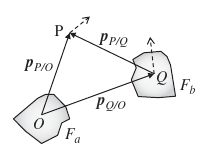
\includegraphics[width=0.25\textwidth, keepaspectratio]{figuras/figure1.5-1.png}
    \label{fig1.5-1}
    \caption{Velocity and acceleration in moving frames.}
\end{figure}

Starting from the left-hand side of Equation (1.5-2), the first two terms are velocities in \(F_{a}\) but the last term involves the position of \(P\) relative to a fixed point in \(F_{b}\), with the derivative taken in \(F_{a}\). Let \(\mathbf{v}\) with an appropriate subscript represent a velocity vector. Then, by applying the equation of Coriolis, Equation (1.5-2) gives
\begin{equation}
    \mathbf{v}_{P/a} = \mathbf{v}_{Q/a} + \left( \mathbf{v}_{P/b} + \mathbf{\omega}_{b/a}\!\times\!\mathbf{p}_{P/Q} \right) \tag{1.5-3}
\end{equation}
Note that (1.5-3) can be written as:
\begin{equation*}
    \mathbf{v}_{P/a} = \mathbf{v}_{P/b} + \left( \mathbf{v}_{Q/a} + \mathbf{\omega}_{b/a}\!\times\!\mathbf{p}_{P/Q} \right),
\end{equation*}
where the term in parentheses is the velocity in \(F_{a}\) of a fixed point in \(F_{b}\) that is instantaneously coincident with \(P\) and is called the \textit{transport velocity of \(P\) in \(F_{a}\)}.

As an application of Equation (1.5-3), let \(F_{a}\) be an inertial reference frame and \(F_{b}\) a body moving with respect to the reference frame. assume that a navigator on the moving body determines, from an onboard inertial navigation system, his velocity in the inertial reference frame \(\mathbf{v}_{Q/a}\) and his inertial angular velocity \(\mathbf{\omega}_{b/a}\). Also, using a radar set, he measures the velocity \(\mathbf{v}_{P/b}\), of \(P\) in \(F_{b}\) and the position \(\mathbf{p}_{P/Q}\) of \(P\) with respect to \(Q\). He can then use the Equation (1.5-3), with appropriately chosen coordinate systems, to calculate the velocity of the object in the inertial reference frame and, knowing the equation of motion in the inertial frame, predict its trajectory.

We next find the acceleration of \(P\) by taking derivatives of (1.5-3) in \(F_{a}\). Starting from left, the first two terms are velocities in \(F_{a}\) and these become accelerations in \(F_{a}\). The third term is a velocity in \(F_{b}\) and must be differentiated by the equation of Coriolis. The last term involving a cross-product can be differentiated by the ``product rule,'' and the derivative of angular velocity is an angular acceleration vector, denoted by \(\mathbf{\alpha}\). Therefore, denoting translational acceleration by \(\mathbf{a}\), (1.5-3) yields
\begin{equation*}
    \mathbf{a}_{P/a} = \mathbf{a}_{Q/a} + \left(\mathbf{a}_{P/b} + \mathbf{\omega}_{b/a}\!\times\!\mathbf{v}_{P/b}\right) + {{\mathbf{\alpha}_{b/a}}\!\times\!{\mathbf{p}_{P/Q}}} + {\mathbf{\omega}_{b/a}}\!\times\!{\left({\mathbf{v}_{P/b}} + {{\mathbf{\omega}_{b/a}}\!\times\!{\mathbf{p}_{P/Q}}}\right)}
\end{equation*}

Regrouping terms, we get
\begin{equation*}
    \mathbf{a}_{P/a} = \mathbf{a}_{P/b} + \overbrace{\mathbf{a}_{Q/a} + {{\mathbf{\alpha}_{b/a}}\!\times\!{\mathbf{p}_{P/Q}}} + \underbrace{{{\mathbf{\omega}_{b/a}}\!\times\!{\left({\mathbf{\omega}_{b/a}}\!\times\!{\mathbf{p}_{P/Q}}\right)}}}_{\text{Centripetal Acceleration}}}^{\text{Transport  Acceleration of \(P\) in Frame \(a\)}} + \underbrace{{2\mathbf{\omega}_{b/a}\!\times\!\mathbf{v}_{P/b}}}_{\text{Coriolis Acceleration}} \tag{1.5-4}
\end{equation*}

Here, the names \textit{total acceleration} and \textit{relative acceleration} apply to the reference and secondary frames, respectively. If \(P\) were fixed in \(F_{b}\) the first and last right-hand-side terms would vanish, leaving only  the \textit{transport acceleration}; this is defined as the acceleration in \(F_{a}\) of a fixed point in \(F_{b}\) that is instantaneously coincident with \(P\). As could be anticipated, the transport acceleration term contains the effects of the motion of \(F_{b}\) in terms of the acceleration of the reference point \(Q\) and the angular acceleration and angular velocity of the frame [see (1) for more detail of the centripetal term]. A comparison of the acceleration equation with the velocity equation shows that a new type of term has appeared, namely the \textit{Coriolis acceleration}. The significance of Coriolis acceleration is examined in the following subsection.

\paragraph{Example 1.5-1. Sensor Fixed in A Moving Body.} A sensor (e.g., accelerometer, radar, etc.) fixed to a rigid vehicle has no velocity or acceleration in that frame, to according to Equation (1.5-3) or (1.5-4) only the transport term in these equations is nonzero. Sensor motion must often be related analytically to the motion of the vehicle cm (or perhaps some other fixed point). For example, with the same notation as Equation (1.5-4), an accelerometer at position \(P\), with position vector \(\mathbf{p}_{P/Q}\) relative to the point \(Q\), has an acceleration given by
\begin{equation*}
    {\mathbf{a}_{P/a}} = {\mathbf{a}_{Q/a}} + {\mathbf{\alpha}_{b/a}}\!\times\!{\mathbf{p}_{P/Q}} + {\mathbf{\omega}_{b/a}}\!\times\!\left({\mathbf{\omega}_{b/a}}\!\times\!{\mathbf{p}_{P/Q}}\right),
\end{equation*}
where \(a\) and \(b\) denote, respectively, the reference and vehicle frames.

\subsection{Acceleration Relative to Earth}

This book is concerned with the motion of aerospace vehicles over the Earth, and acceleration relative to Earth is the starting point for equations of motion. Using the results of the previous subsection, let \(F_{a}\) become an inertial frame \(F_{i}\) and \(F_{b}\) become the rigid Earth frame \(F_{e}\). Let the points \(Q\) and \(O\) coincide, at Earth's cm (Earth is assumed to have no translational acceleration) so that the acceleration \(\mathbf{a}_{Q/a}\) vanishes and \(\mathbf{p}_{P/Q}\) is a geocentric position vector. Earth's angular velocity is closely constant and so the derivative os \(\mathbf{\omega}_{b/a}\) vanishes. This leaves only the relative acceleration, centripetal acceleration, and Coriolis acceleration terms and gives the fundamental equation, relating true (inertial) acceleration to relative acceleration, that we will use in Section 1.7 to apply Newton's laws to motion of a point \(P\) over Earth:
\begin{equation*} \tag{1.5-5}
    {\mathbf{a}_{P/i}} = {\mathbf{a}_{P/e}} + {\mathbf{\omega}_{e/i}}\!\times\!\left({\mathbf{\omega}_{e/i}}\!\times\!{\mathbf{p}_{P/O}}\right) + 2\mathbf{\omega}_{e/i}\!\times\!\mathbf{v}_{P/e}
\end{equation*}
For a particle of mass \(m\) at \(P\), the relative acceleration \(\mathbf{a}_{P/e}\) corresponds to an ``apparent force'' on the particle and produces the trajectory observed by a stationary observer on Earth. The true acceleration \(\mathbf{a}_{P/i}\), corresponds to ``true'' forces (e.g., mass attraction,  drag); therefore, writing (1.5-5) in terms of force,
\begin{equation*}
    \text{Apparent force} = \text{true force} - m \left[{\mathbf{\omega}_{e/i}}\!\times\!\left({\mathbf{\omega}_{e/i}}\!\times\!{\mathbf{p}_{P/O}}\right)\right] - m \left( 2{\mathbf{\omega}_{e/i}}\!\times\!{\mathbf{v}_{P/e}}\right)
\end{equation*}
The second term on the right is the \textit{centrifugal force}, directed normal to the angular velocity vector. The third term is usually referred to as the \textit{Coriolis force} and will cause a ballistic trajectory over Earth to curve to the left or right.

The true force is the sum of the \textit{contact forces}, say \(F\), and the mass attraction of \textit{Earth's gravitational field}, \(m\mathbf{G}\) (see next section). The Earth gravity vector is \(\mathbf{g} = \mathbf{G} - \text{centripetal acceleration}\) (see next section), so Equation (1.5-5) is often written (for a body of mass \(m\)) as
\begin{equation*} \tag{1.5-6}
    \mathbf{a}_{P/e} = \frac{F}{m} + g - {2 \mathbf{\omega}_{e/i}}\!\times\!{\mathbf{v}_{P/e}}
\end{equation*}

An often-quoted example of the Coriolis force is the circulation of winds around a low-pressure area (a cyclone) on Earth. The true force is radially inward along the pressure gradient. In the Northern Hemisphere, for example, Earth's angular velocity vector points outward from Earth's surface and, whichever way the velocity vector \({\mathbf{v}_{P/e}}\) is directed, the Coriolis force is directed to the right of \({\mathbf{v}_{P/e}}\). Therefore, in the Northern Hemisphere the winds spiral inward in a counterclockwise direction around a cyclone.

The Coriolis acceleration is also significant in high-speed flight; it is zero for an aircraft flying due North or South at the equator and reaches its maximum value at the poles or for flight due East or West at any latitude. Its significance can be estimated by equating its value to the centripetal acceleration, in low, constant-altitude flight, at \(45^{\circ}\) latitude, and solving for the speed over Earth:
\begin{align*}
    &2 \! \begin{vmatrix}{\mathbf{\omega}_{e/i}}\end{vmatrix} \begin{vmatrix}{\mathbf{v}_{cm/e}}\end{vmatrix}\sin\!{\left({45^{\circ}}\right)} = {\begin{vmatrix}{\mathbf{v}_{cm/e}}\end{vmatrix}^{2}} / {r_{E}} \\
    &\begin{vmatrix}{\mathbf{v}_{cm/e}}\end{vmatrix} = {\sqrt{2}}{r_{E}} \begin{vmatrix} {\mathbf{\omega}_{e/i}}\end{vmatrix} \approx 657\text{m/s} \left(2156\text{ft/s}\right)
\end{align*}

At this speed the Coriolis acceleration is equal to the centripetal acceleration and is very small compared to \(\mathbf{g}\) bu causes a position error that grows quadratically with time.

\subsection{Gravitation and Accelerometers}

The basic principle usend in nearly all accelerometers is measurement, indirectly, of the force \(\mathbf{F}\), that must be applied (mechanically or by means of a magnetic or electrostatic field) to prevent a known ``proof'' mass from accelerating with respect to its instrument case when the case is being aceclerated. Thus, apart from a small transient and/or steady-state error determined by the dynamics of the proof mass ``rebalancing'' servo and the type of the acceleration signal, the acceleration of the proof mass is the same as the acceleration of the case. An accelerometer is usually a single-axis device, but here we will write vector equations for the acceleration experienced by the accelerometer. The gravitational field always acts on the proof mass, \(m\), and so the acceleration, \(\mathbf{a}\), of the proof mass id given by the vector sum:
\begin{equation*}
    \mathbf{a} = \dfrac{\mathbf{F}}{m} + \mathbf{G} \equiv \mathbf{f} + \mathbf{G}.
\end{equation*}
where \(\mathbf{F}/m\) is the force per unit mass applied to the proof mass, called the specific force, \(\mathbf{f}\). The accelerometer calibration procedure determines the \textit{scale factor}, \(s\), realting the output quantity to the specific force, and so the accelerometer equation is
\begin{equation*} \tag{1.6-28}
    \text{Accelerometer output} = s \mathbf{f} = s \left(\mathbf{a} - \mathbf{G} \right)
\end{equation*}

Equation (1.6-28) shows that an accelerometer is basically a specific force measuring device. When acceleration must be measured precisely (as in inertial navigation), an accurate model of \(\mathbf{G}\) (as a function of position) is essential. In other, lower precision applications the accelerometer ``bias'' of \(\mathbf{G}\) is not a limitation.

When an accelerometers'a sensitive axis is horizontal, the bias is zero. When an accelerometer, with geocentric position vector \(\mathbf{p}\), is stationary with respect to Earth, its acceleration and specific force reading are given by
\begin{align*}
    \mathbf{a} &= {\mathbf{\omega}_{e/i}}\!\times\!\left({\mathbf{\omega}_{e/i}}\!\times\!{\mathbf{p}}\right) \\
    \mathbf{f} &= \mathbf{a} - \mathbf{G} = -\!{\mathbf{g}} \tag{1.6-29}
\end{align*}

At a different position from the calibration location, the accelerometer could be corrected to the local gravity, but if acceleration is to be calculated accurately, a correction would have to be aplied for the different (in general) centripetal acceleration. For accelerometers in motion over Earth, we must evaluate a transport acceleration to relate accelerometer acceleration to vehicle acceleration, as shown in Chapter 4 for the normal-acceleration control augmentation system.
